\documentclass[10pt]{beamer}
\usepackage[utf8]{inputenc}
\usetheme{default}
\usecolortheme{dove}
\usepackage{textpos}
\usepackage{grid-system}
\usepackage[T1]{fontenc}

\AtBeginSection[]
{
  \begin{frame}<beamer>
    \frametitle{Übersicht}
    \tableofcontents[currentsection]
  \end{frame}
}

% TODO:
% - Hinweis auf Cryptoparty Computerwerk?
% - "Vision" aus 2015-10-04_VeganBrunch einarbeiten, wo sinnvoll
% - Welche Router kaufen?

% TODO: Vielleicht kann man die Titelfolie noch ein wenig aufpeppen?
% - Hintergrundbild?
% - Warum ist unser Footer mitten auf der Seite?
%   -> Footer ohne Logo nach unten
%   -> Großes Logo in die Mitte
\title{Freifunk Darmstadt}
\author{}
\institute[Inst.]{eine Initiative des Chaos Darmstadt e.V.}
\date{\footnotesize 19. Februar 2016}

\begin{document}
  \addtobeamertemplate{frametitle}{}{
    \begin{textblock*}{0cm}(\textwidth-0.85cm,-0.85cm)
      %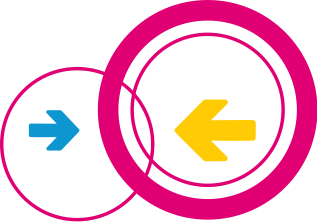
\includegraphics[height=1cm]{images/logo}
      \begin{figure}[h]
        \def\svgwidth{1.5cm}
        \input{logo.pdf_tex}
      \end{figure}

    \end{textblock*}
  }

  \begin{frame}
    \centering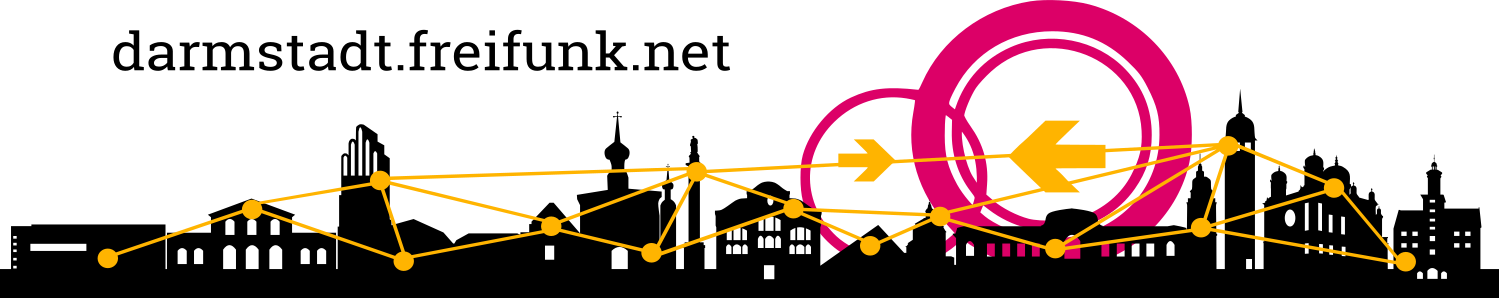
\includegraphics[width=\textwidth]{images/logo-skyline}
    \maketitle
  \end{frame}

  \begin{frame}{Übersicht}
    \tableofcontents
  \end{frame}

  \section{Was ist Freifunk?}
    \begin{frame}{Was ist Freifunk?}
      \begin{center}
        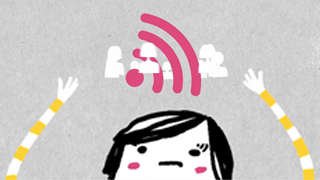
\includegraphics[width=0.5\textwidth]{images/up}
      \end{center}
      Wie wäre es, wenn\ldots
      \begin{itemize}
        \pause
        \item online jeder mit jedem kommunizieren könnte\pause, \textit{\textbf{ohne eine Firma}, bei der man sich anmelden muss?}
        \pause
        \item wir unsere eigenen Dienste betreiben könnten\pause,  \textit{\textbf{ohne} auf einen \textbf{zentralen kommerziellen Anbieter} angewiesen zu sein?}
        \pause
        \item Kommunikation jederzeit möglich ist\pause, \textit{auch wenn unsere herkömmliche \textbf{Infrastruktur ausfällt}}
      \end{itemize}
    \end{frame}

    \begin{frame}{Prinzipien}
      \begin{centering}
        \large{\textbf{Wie sollte die Infrastruktur für unsere tägliche Kommunikation beschaffen sein?}}
      \end{centering}
      \pause
      \vfill
      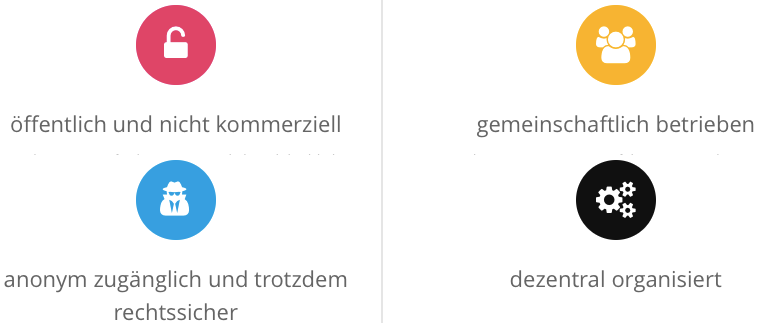
\includegraphics[width=1.1\textheight]{images/principles}
    \end{frame}

    \begin{frame}{Freifunk: offen und öffentlich}
      \begin{columns}[c]
        \begin{column}{5cm}
          
\includegraphics[width=\textwidth]{images/open}
          \newline \tiny \url{https://flickr.com/photos/29355306@N06/15613972489}
        \end{column}
        \begin{column}{7cm}
          \begin{itemize}
            \item freie, ungehinderte Teilnahme an Betrieb und Ausbau des Netzes $\Rightarrow$ \textbf{Mitmachnetz}
            \item im Besitz der \textit{Gemeinschaft}
            \item \textit{anonymer, unzensierer Zugang} zu Netz und Diensten
            \item \textit{keine Unterscheidung} nach Ort oder Geldbeutel
            \item \textit{Datensparsamkeit}
            \item \textbf{Unterstützung jederzeit willkommen!}
          \end{itemize}
        \end{column}
      \end{columns}
    \end{frame}

    \begin{frame}{Was ist Freifunk?}
      \large \textbf{Deutschlandweite Initiative für \emph{freie} Netze.}
      \pause
      \begin{center}
        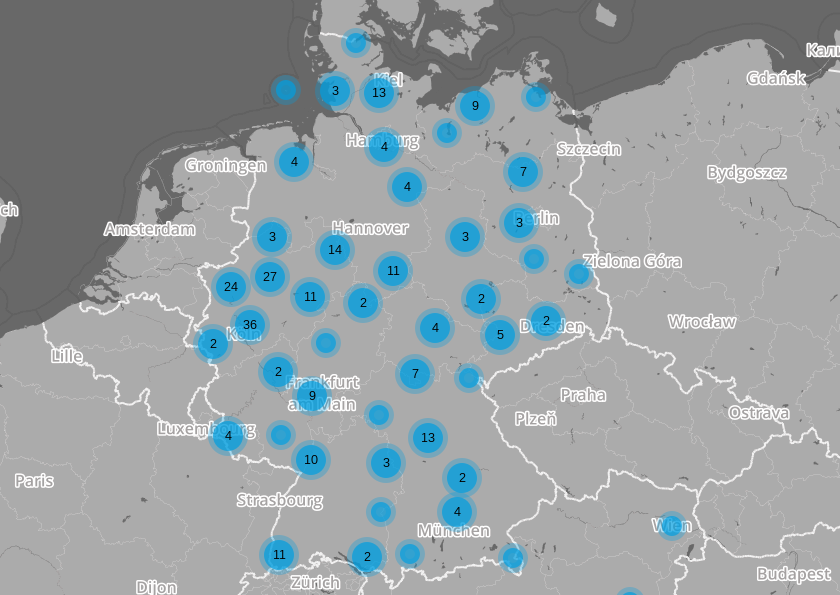
\includegraphics[height=12em]{images/2016-02-17_map-de}
      \end{center}
      \begin{itemize}
        \item 275 lokale Gruppen
        \item ca. 29.700 offene Zugangspunkte\footnote{\url{http://freifunk.net/map/map.html}}
        \item Teil einer weltweiten Bewegung für offene und freie Netze
      \end{itemize}
    \end{frame}

    \begin{frame}{Ziele von Freifunk}
      \begin{columns}[T]
        \begin{column}{5cm}
          \begin{itemize}
            \item \textbf{Verständnis von Kommunikationsnetzen} sowie deren Auswirkungen auf die Gesellschaft fördern
            \item Teilnahme der Bevölkerung an \textbf{Forschung und Aufbau} dezentraler Netze
            \item unser \textbf{Wissen und Software} öffentlich zugänglich machen
            \item Beteiligung an politischen Prozessen, um \textbf{rechtliche Voraussetzungen} für freie Netze zu schaffen
          \end{itemize}
        \end{column}
        \begin{column}{5cm}
          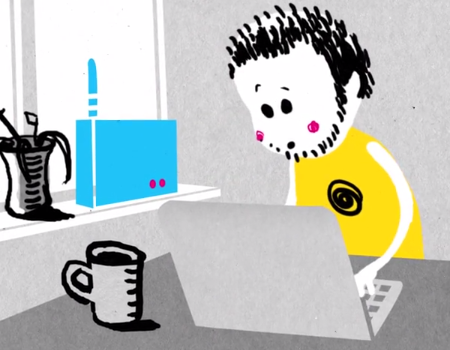
\includegraphics[height=10em]{images/install}
        \end{column}
      \end{columns}
    \end{frame}

    \begin{frame}{Wie sieht so ein freies Netz aus?}
      \begin{center}
        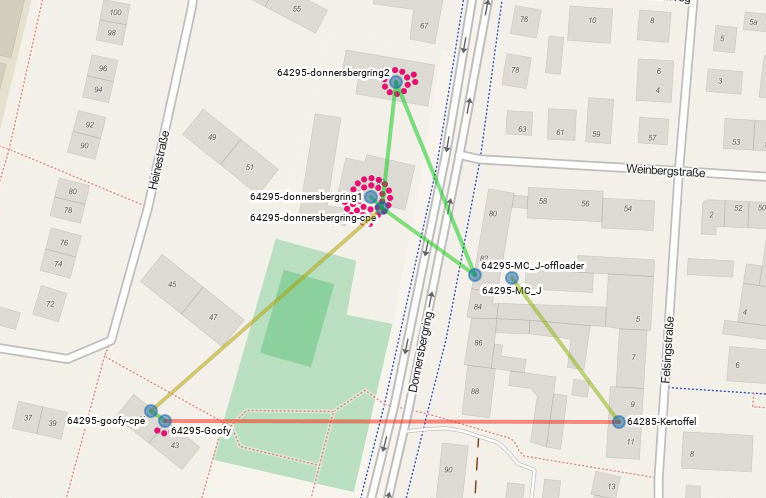
\includegraphics[height=6cm]{images/2016-02-17_donnersbergring}
        \vfill Donnersbergring
      \end{center}
    \end{frame}

    \begin{frame}{Wie sieht so ein freies Netz aus?}
      \begin{center}
        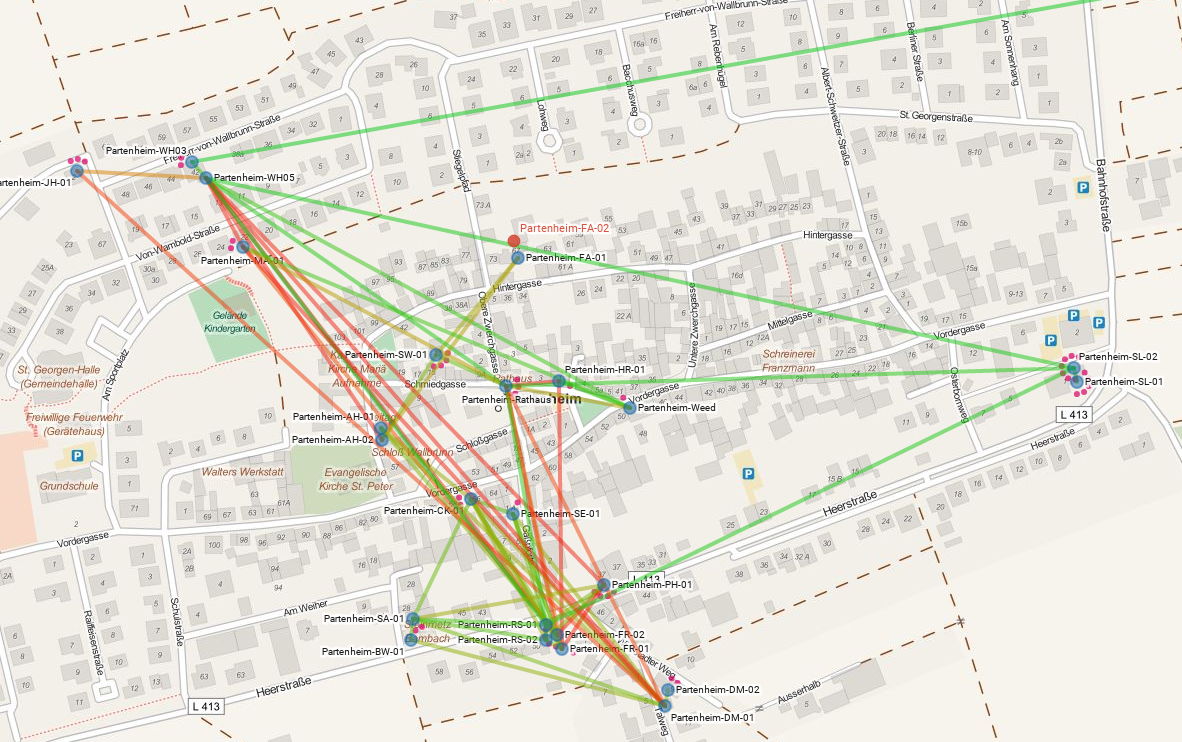
\includegraphics[height=6cm]{images/2015-10_partenheim-map}
        \vfill Partenheim bei Mainz
      \end{center}
    \end{frame}

    \begin{frame}{Wie sieht so ein freies Netz aus?}
      \begin{center}
        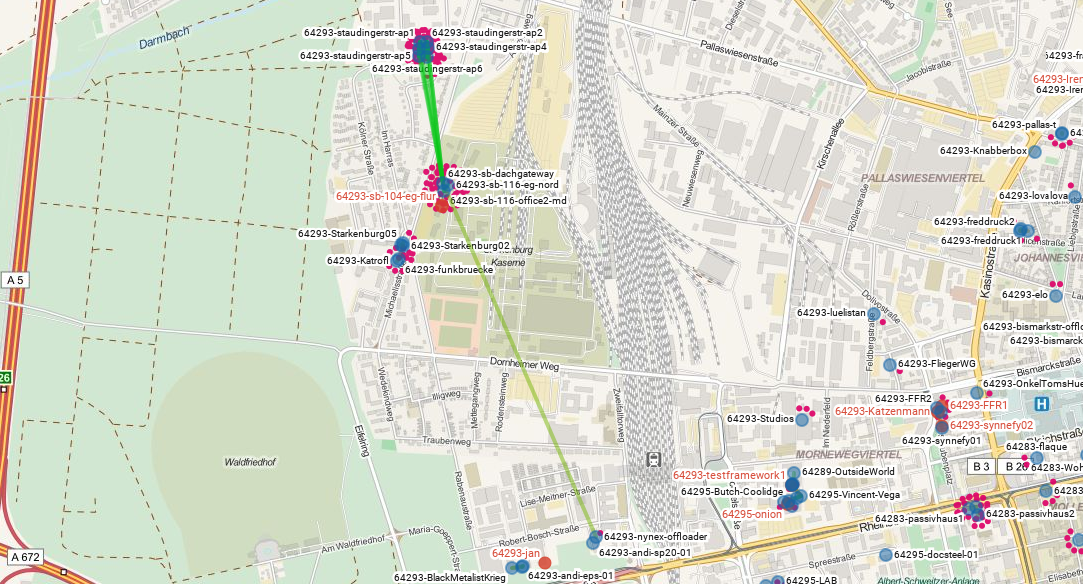
\includegraphics[height=6cm]{images/2016-02-17_starkenburk-link}
        \vfill Versorgung der Geflüchteten
        \vfill \small Starkenburgkaserne und Staudinger Strße
      \end{center}
    \end{frame}

    \begin{frame}{Warum ein freies Netz?}
      \vfill
      \begin{center}
        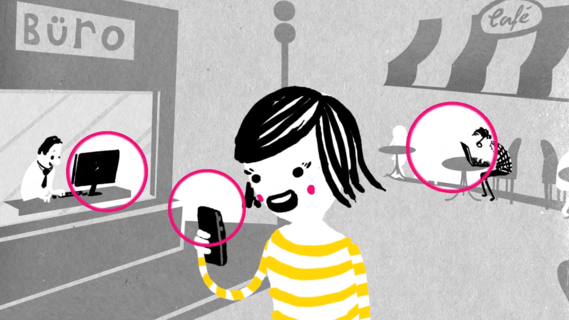
\includegraphics[width=5.5cm]{images/verbindet}
      \end{center}

      \begin{itemize}
        \item \emph{gleichberechtigt} Netzwerkdienste anbieten und nutzen
        \begin{itemize}
          \item Telefonieren und Chatten (z.B. Tox, Ricochet, Mumble)
          \item dezentrales Social-Media (z.B Diaspora, Twister)
          \item lizenzfreies Community-Radio (in Planung, hilf uns dabei!)
          \item Austausch von Dateien und Medien
          \item lokale Webseiten, Nachrichten, Blogs
          \item \ldots
        \end{itemize}
        \item Internetzugänge \emph{teilen}
        \item \emph{krisensichere} Netzwerktopologie
      \end{itemize}
      \vfill
    \end{frame}

  \section{Wie funktioniert Freifunk?}

    \begin{frame}{Ohne Freifunk}
      \begin{center}
        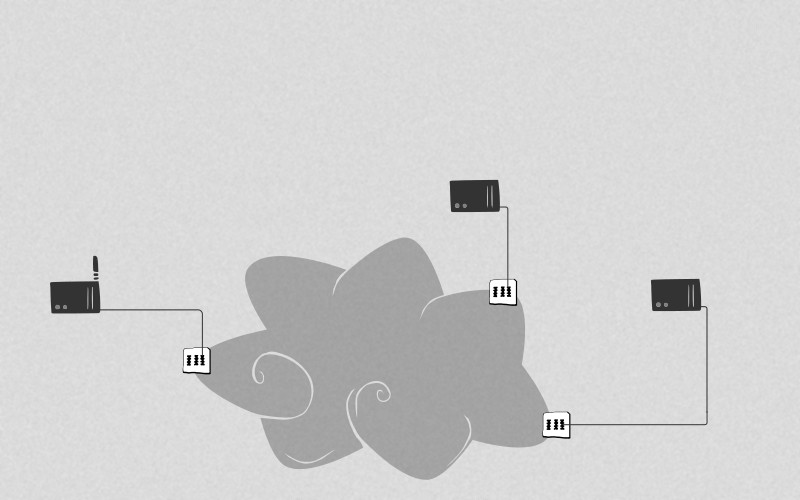
\includegraphics[height=6cm]{images/network_1}\\
        \vspace{1em}
        geschlossene WLAN-Netze, die nicht miteinander kommunizieren
        \vspace{1em}
      \end{center}
    \end{frame}

    \begin{frame}{Mit Freifunk}
      \begin{center}
        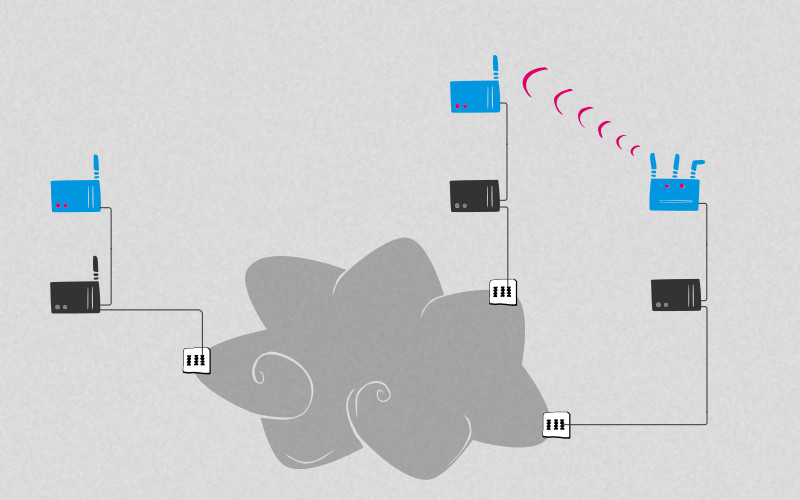
\includegraphics[height=6cm]{images/network_2}\\
        \vspace{1em}
        Freifunkknoten bauen ein lokales Netz auf
        \vspace{1em}
      \end{center}
    \end{frame}

    \begin{frame}{Verminderung der digitalen Kluft}
      \begin{center}
        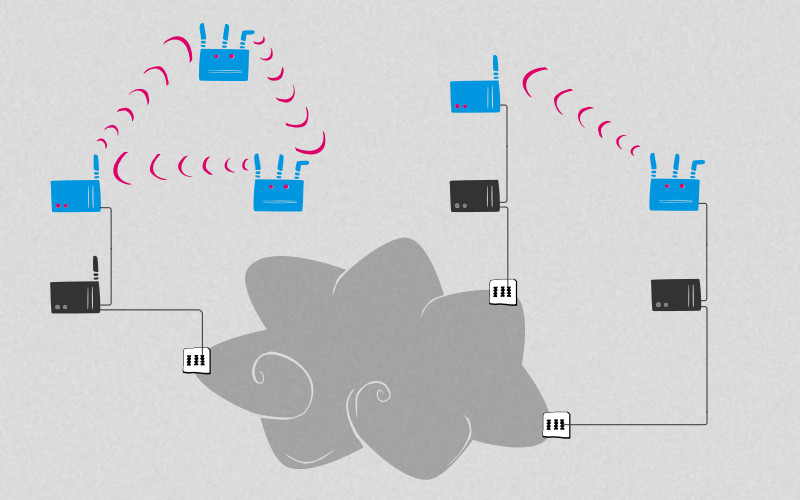
\includegraphics[height=6cm]{images/network_3}\\
        \vspace{1em}
        neue Knoten ohne Internetzugang
        \vspace{1em}
      \end{center}
    \end{frame}

    \begin{frame}{Das Heimnetz bleibt privat}
      \begin{center}
        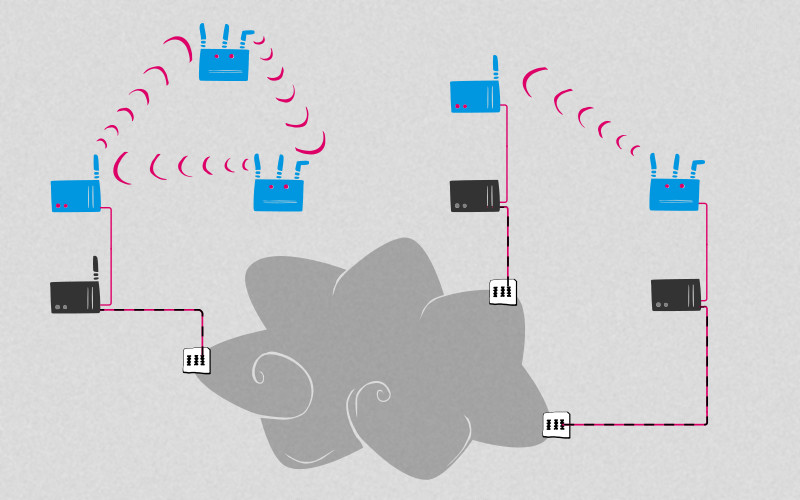
\includegraphics[height=6cm]{images/network_4}\\
        \vspace{1em}
        eigenes Heimnetz und Freifunk-Netz sind getrennt
        \vspace{1em}
      \end{center}
    \end{frame}

    \begin{frame}{Zugang zum Internet}
      \begin{center}
        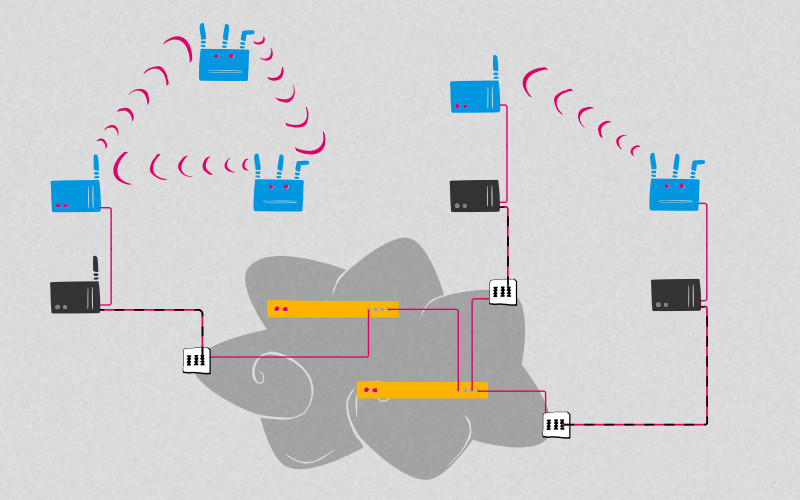
\includegraphics[height=6cm]{images/network_5}\\
        \vspace{1em}
        übers Gateways ins Internet
        \vspace{1em}
      \end{center}
    \end{frame}

    \begin{frame}{Sicherheit im Freifunk-Netz}
      \begin{columns}[c]
        \begin{column}{5cm}
          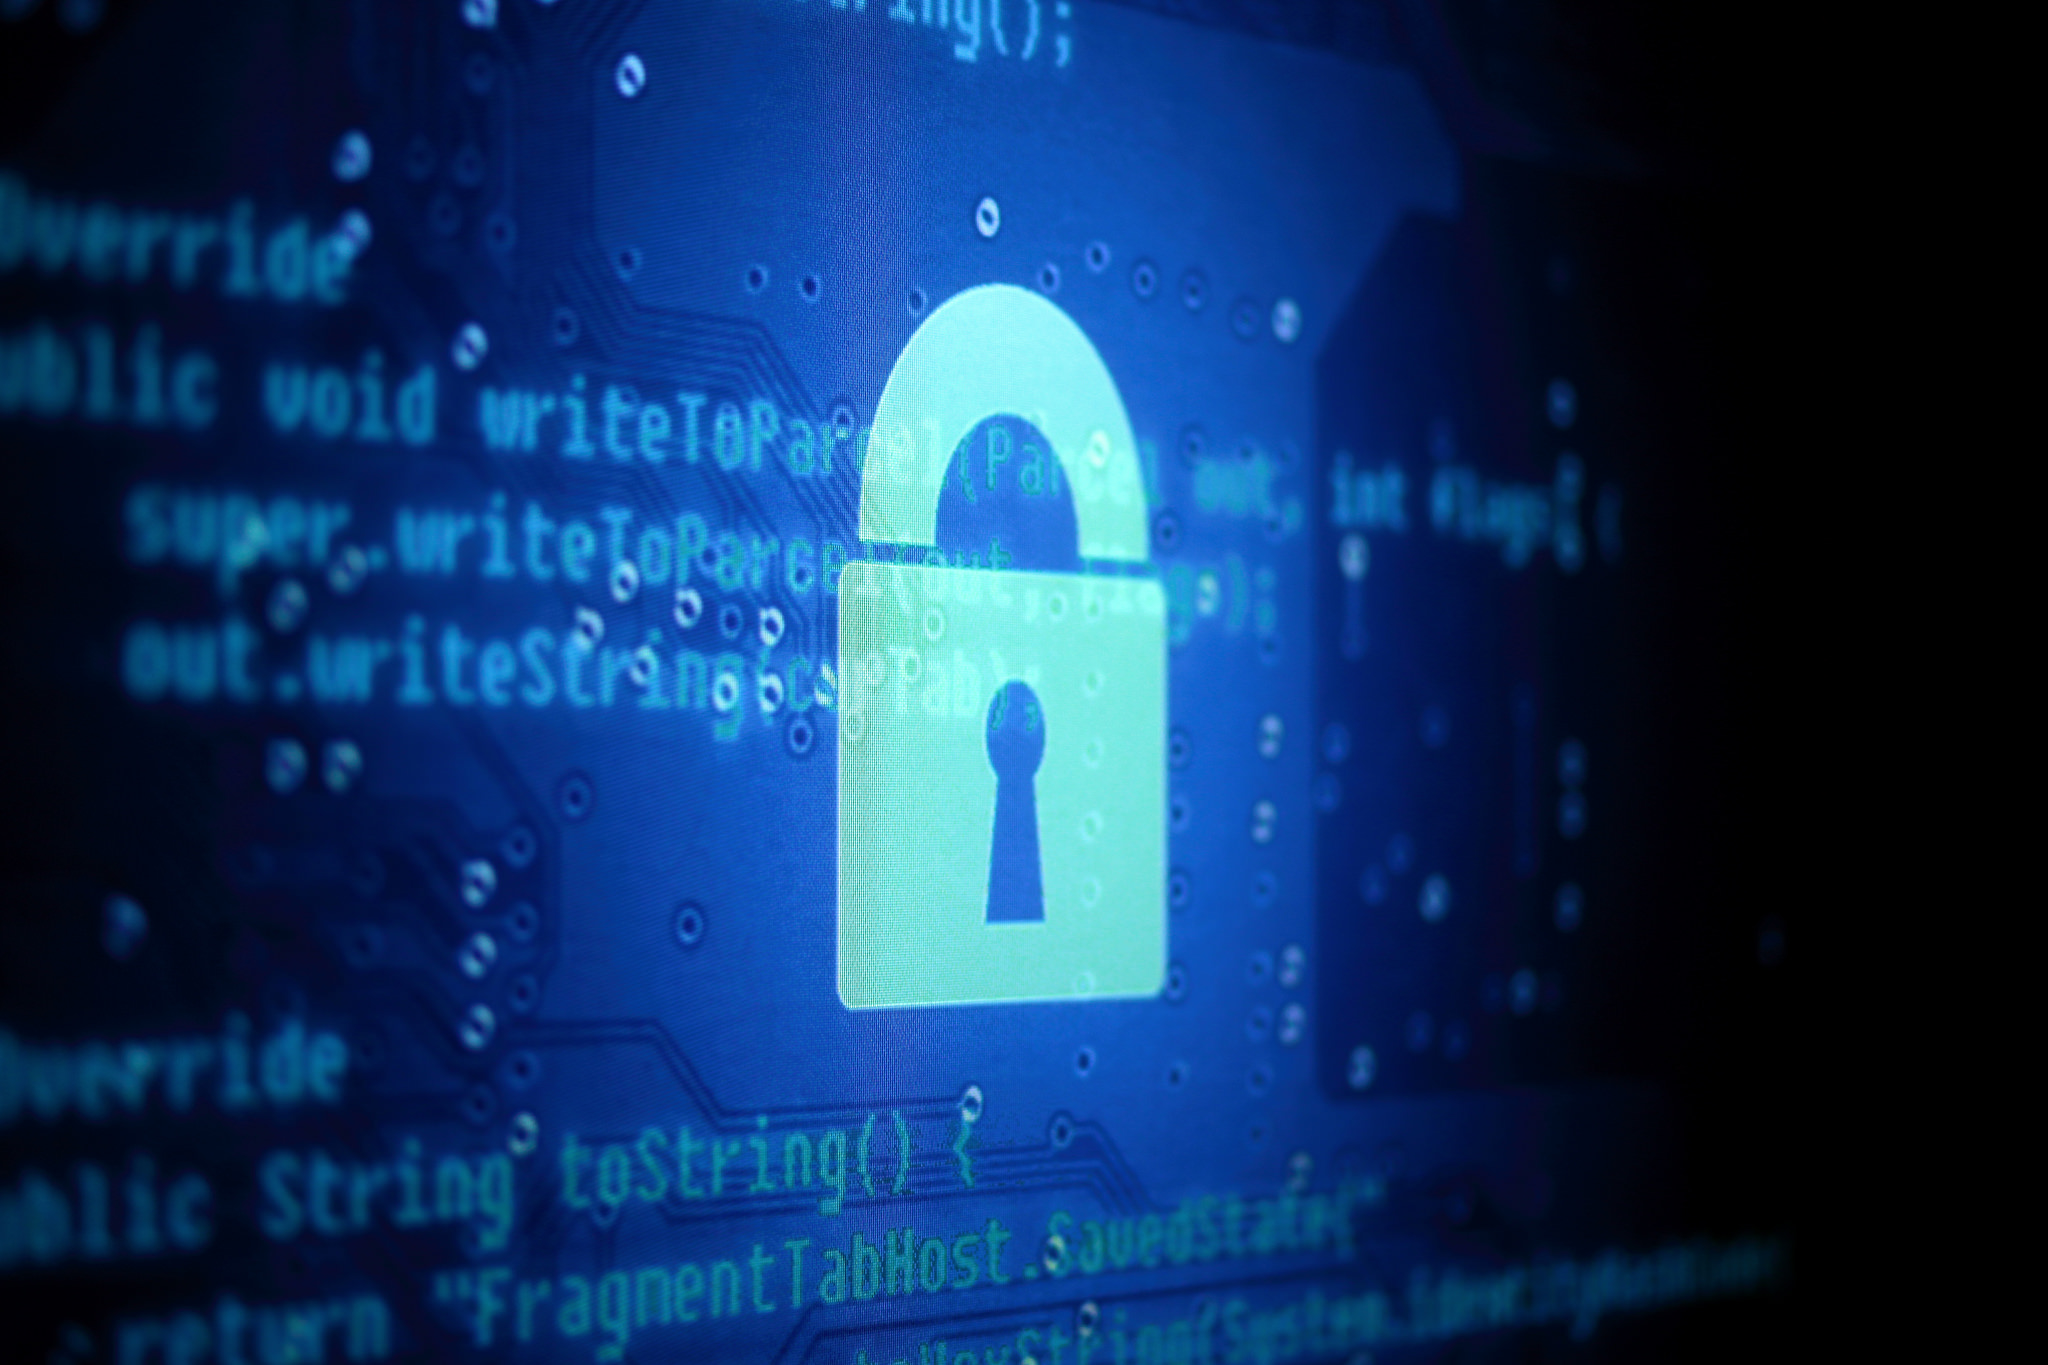
\includegraphics[width=\textwidth]{images/lock}
          \newline \tiny \url{https://www.flickr.com/photos/yusamoilov/13334048894}
        \end{column}
        \begin{column}{7cm}
          \begin{itemize}
            \item Freifunk als freies Netz bietet keinen Schutz
            \item WLAN ist nicht verschlüsselt
            \item unverschlüsselte Kommunikation kann mitgelesen werden
            \pause
            \item Daher: vertrauliche Daten nur mit Ende-zu-Ende-Verschlüsselung übertragen!
            \item auf http\textbf{s} achten (grünes Schloss)
          \end{itemize}
        \end{column}
      \end{columns}
      \vfill
      \pause
      \textbf{Fazit:}\\Zentrale Überwachung und Zensur deutlich schwieriger als im Internet, \\
      Benutzer sind selbst verantwortlich für Schutz und Verschlüsselung.
    \end{frame}


  \section{Freifunk in Darmstadt}

    \begin{frame}{1.x Jahre Freifunk Darmstadt}
      \vfill
      \begin{itemize}
        \item 26. Juni 2014: erster Knoten geht online
        \item September 2014: ca. 30 Knoten
        \item heute: 400 Knoten, davon ca. 350 online
        % online nodes: https://api.darmstadt.freifunk.net/alfred/nodeinfo-statistics.json
        % all nodes: https://map.darmstadt.freifunk.net/data/nodes.json

        % TODO: Bandbreiten-Porn (XXX GB/Monat)
      \end{itemize}
      \begin{center}
        % TODO: Haben wir eine aktuellere Grafik?
        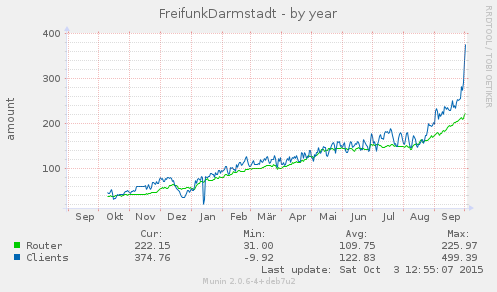
\includegraphics[width=0.8\textwidth]{images/ffda-Okt14-15}
      \end{center}
    \end{frame}

    \begin{frame}{Stand September 2014}
      ca. 30 Knoten
      \begin{center}
        \vfill
        \begin{center}
          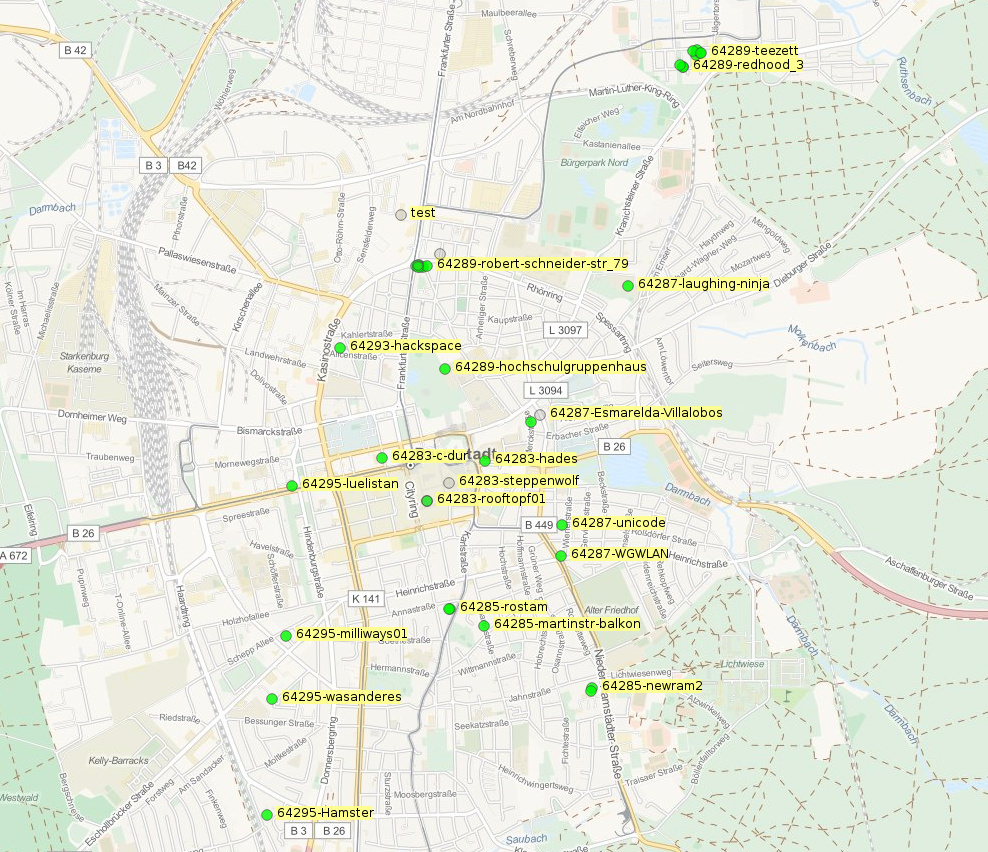
\includegraphics[height=6.5cm]{images/darmstadt-map}
        \end{center}
        \vfill
        \url{https://map.darmstadt.freifunk.net}
      \end{center}
    \end{frame}

    \begin{frame}{Stand Februar 2016}
      ca. 347 Knoten mit täglich über 1000 gleichzeitig aktiven Nutzern
      \begin{center}
        \vfill
        \begin{center}
          \only<1>{
            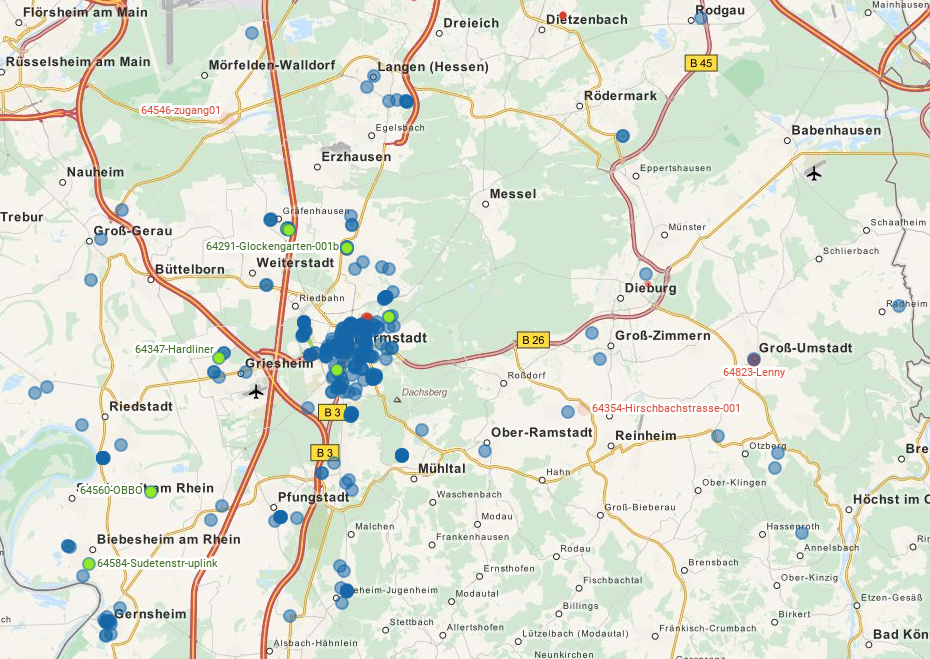
\includegraphics[height=6.5cm]{images/2016-02-17_map-large}
          }
          \only<2>{
            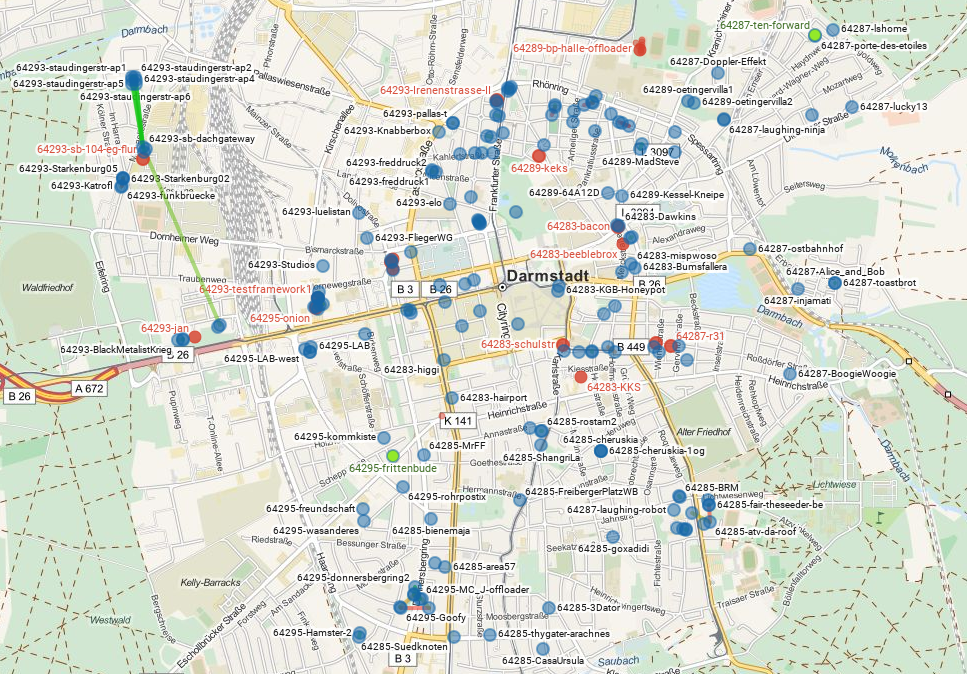
\includegraphics[height=6.5cm]{images/2016-02-17_map-darmstadt}
          }
        \end{center}
        \vfill
        \url{https://map.darmstadt.freifunk.net}
      \end{center}
    \end{frame}

  \section{Aktuelle Aufgaben}

    \begin{frame}{Aktuelle Aufgaben}
      \begin{columns}[T]
        \begin{column}{5cm}
          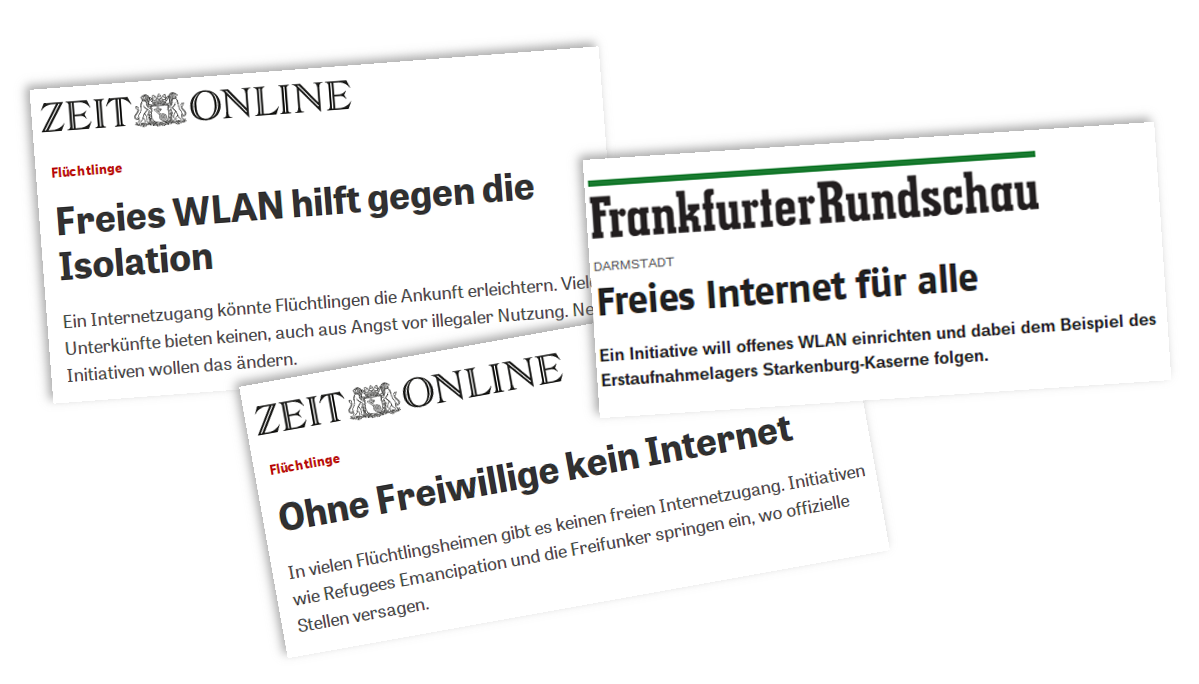
\includegraphics[width=\textwidth]{images/2015-10_presse-fluechtlinge}
          \vspace{1em}
          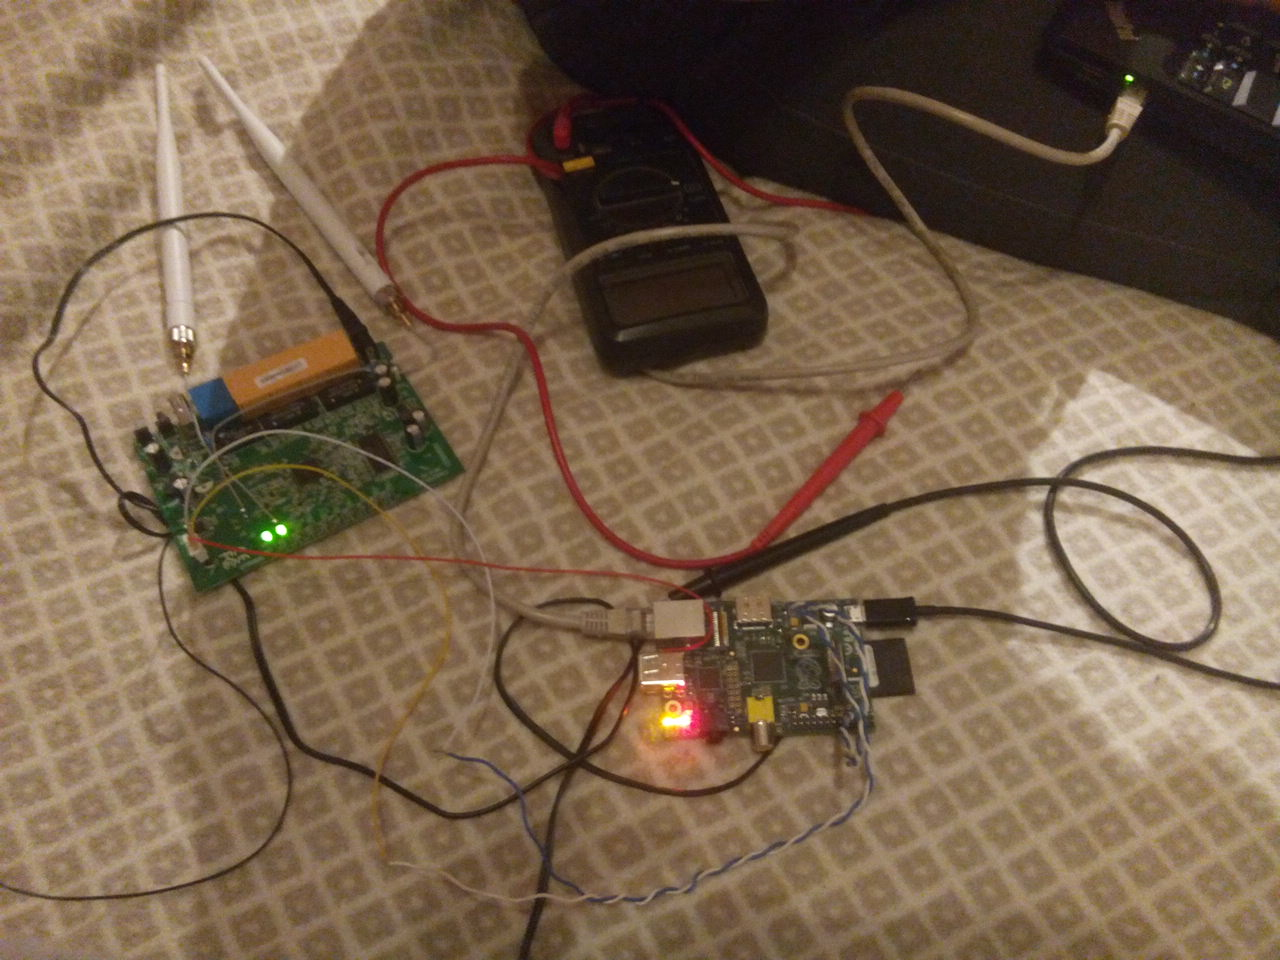
\includegraphics[width=\textwidth]{images/disassemble}
        \end{column}
        \begin{column}{7cm}
        \begin{itemize}
          \item \large Flüchtlingsunterkünfte mit Internet versorgen\\
            % TODO: Diese Liste überarbeiten
            \tiny auch in Eberstadt, Wixhausen, Biebesheim, Stockstadt am Rhein\\
            \tiny hoffentlich bald: Seeheim-Jugenheim, Mühltal
        \end{itemize}
        \begin{itemize}
          \item Freifunk-Software weiterentwickeln
          \item Unterstützer gewinnen
          \item Öffentliche Plätze versorgen
          \item Verbindungen zu anderen Communities aufbauen (ICVPN)
          \item Wireless-Backbone über Darmstadt
        \end{itemize}
        \end{column}
      \end{columns}

    \end{frame}

    \begin{frame}{Wir freuen uns auf Freiwillige}
      \begin{itemize}
        \item 15 Freifunker im Kernteam
        \item viel Arbeit seit Unterbringung der Flüchtlinge
      \end{itemize}
      \vfill
      \hspace{2em}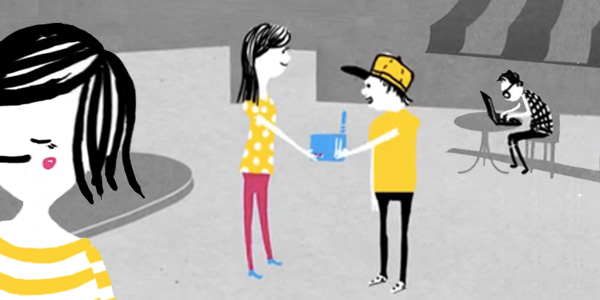
\includegraphics[width=0.6\textwidth]{images/router}
      \vfill
      \begin{itemize}
        \pause
        \item wir treffen uns jeden Montag um 18:30 Uhr
        \item außerdem online im IRC (\#ffda @ hackint.org)
        \item Webchat: \url{https://chat.darmstadt.freifunk.net}
        \item weitere Kontaktmöglichkeiten auf unserer Webseite:\\
        \url{https://darmstadt.freifunk.net/kontakt/}
      \end{itemize}
    \end{frame}

    % TODO: Diese Folie weglassen?
    \begin{frame}{Freifunk Darmstadt: Das wichtigste auf einen Blick}
      \begin{centering}
      \begin{itemize}
        \item Freifunk Darmstadt: eine Initiative des Chaos Darmstadt e.\,V.
        \item Teil einer bundes- und weltweiten Bewegung für offene Netze.
        \item \emph{freies} Netz für lokale Dienste und Internetzugang
        \item \emph{dezentral} aufgabaut und \emph{gemeinschaftlich} betrieben
        \item nicht kommerziell
        \item \emph{krisensichere} Netzwerktopologie durch Mesh-Architektur
      \end{itemize}
      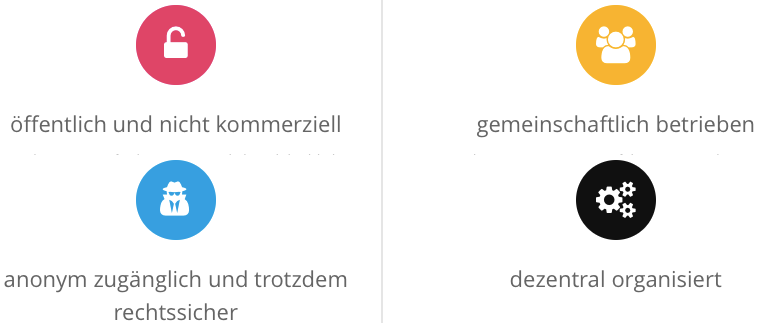
\includegraphics[width=1.0\textheight]{images/principles}$\;$
      \end{centering}
    \end{frame}

    \begin{frame}{Q~\&~A $\rightarrow$ Workshop}
      \vfill
      \centering
      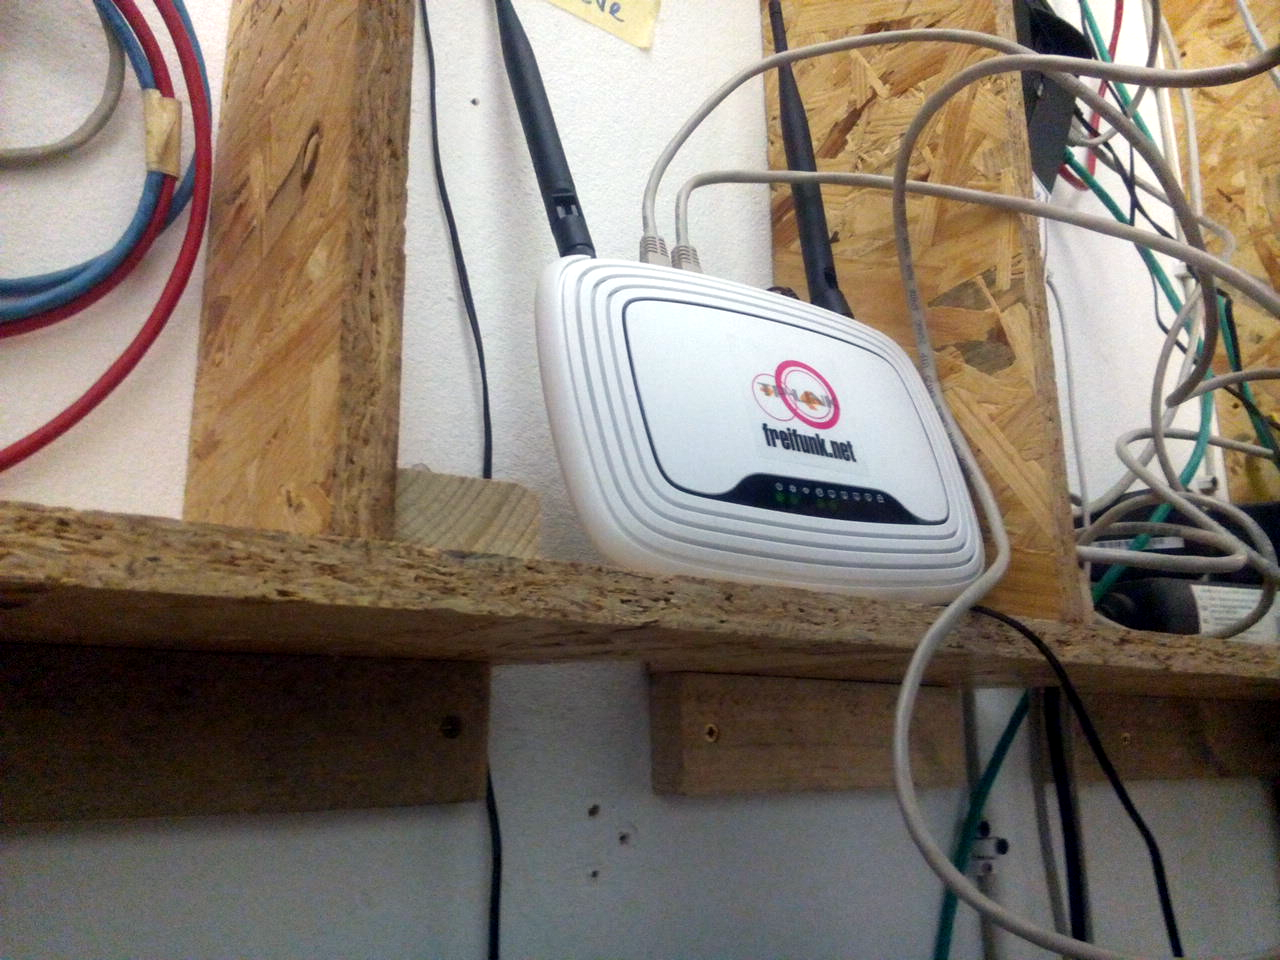
\includegraphics[width=0.7\textwidth]{images/irl_router}
      \vfill
    \end{frame}

\end{document}
